\documentclass[../main/report.tex]{subfiles}
\begin{document}

\section{Power}

The system is powered by a 5V mini usb.
The core design implementation is that this connection feeds electricity towards two voltage regulator circuits.
These, in turn power up the rest of the machine.
The usb connection has a backup solution in the form of a header through which the 5V line passes immediately after entering the pcb.
This is done so that the incoming electricity can easily be probed for voltage level and also so that in case the usb connection fails, an external power supply can be connected to the board.

\begin{figure}[H]
	\centering
	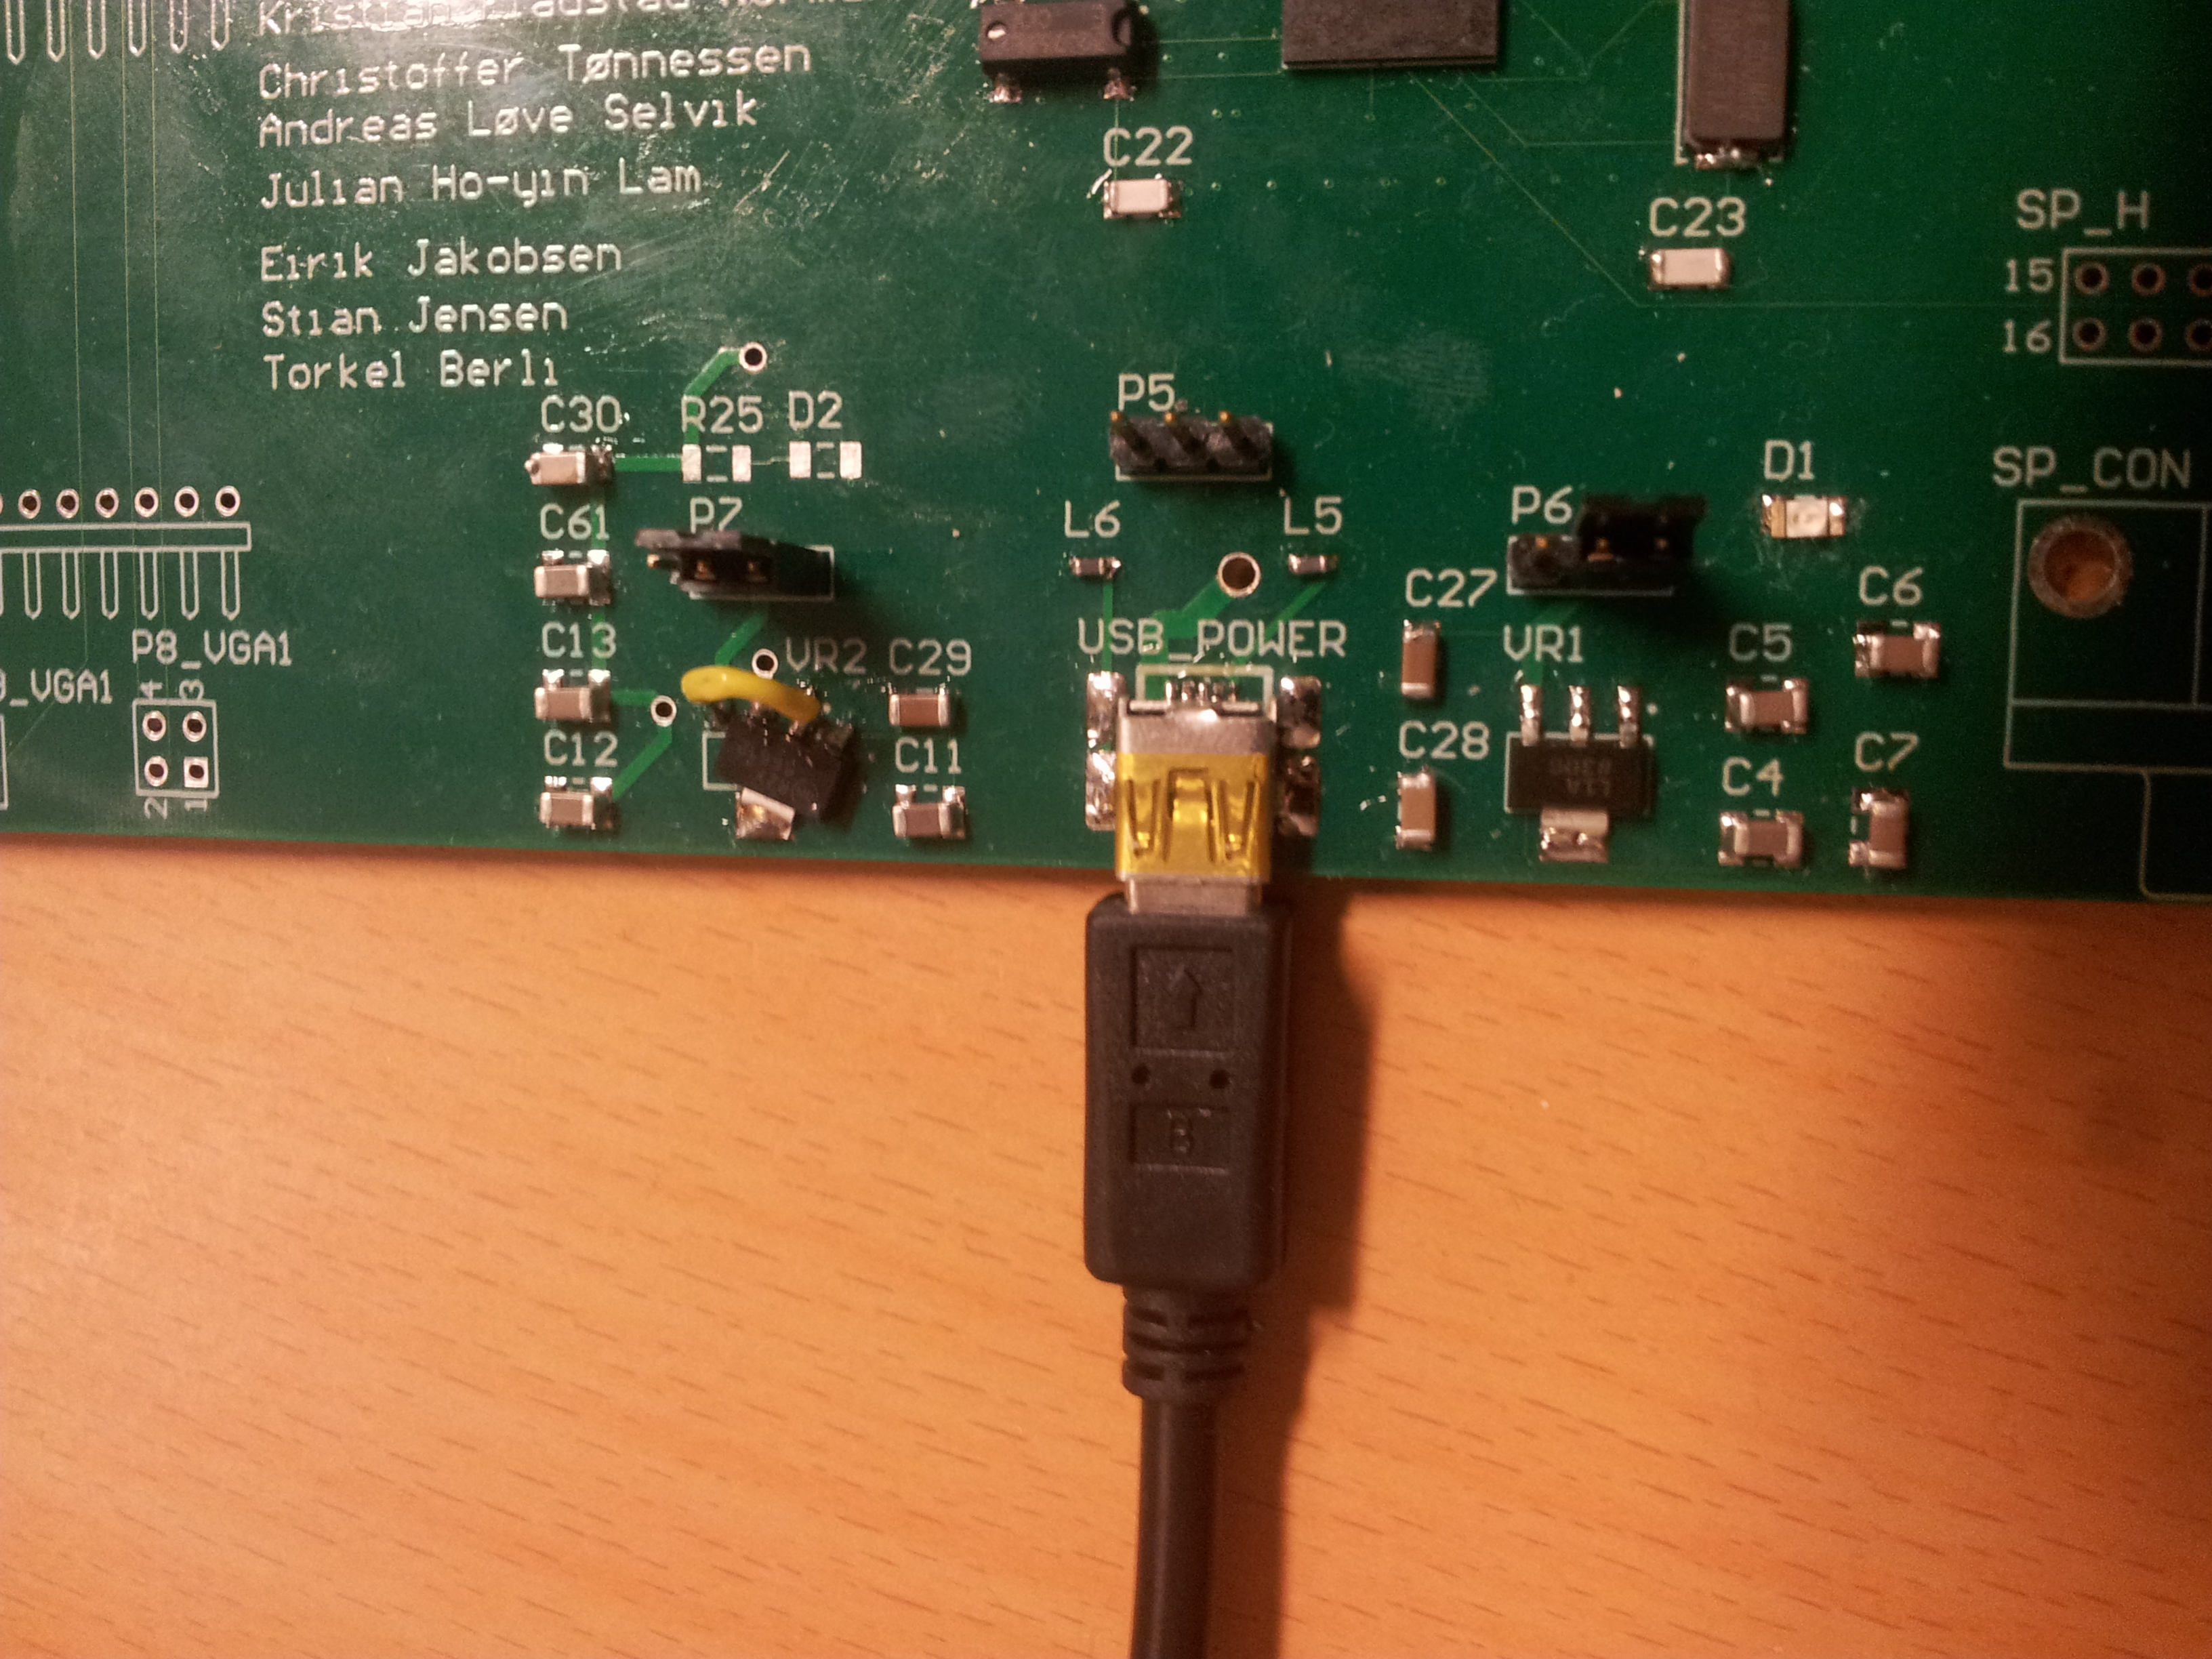
\includegraphics[width=0.65\textwidth]{../pcb/assets/power.jpg}
	\caption{Picture of physical power circuit}
	\label{fig: power picture}
\end{figure}
\todo{If the picture is to stay, should probably crop it a bit}

\end{document}
